\section{Agenti Razionali}
Quando si spiega l’attività umana, è spesso utile fare dichiarazioni come le seguenti: \textit{"Janine ha preso l'ombrello perché lei crede che possa piovere"}. Queste affermazioni fanno uso di una \textbf{psicologia popolare} (folks psychology) che fa riferimento al complesso di teorie, credenze e abilità cognitive e comprende la capacità di intuire il funzionamento della mente e di predirne il comportamento.

L'azione \textit{"Janine ha preso l'ombrello"} a seguito della credenza/intuizione \textit{"lei crede che possa piovere"}.

\subsection{Sistema Intenzionale}
Il filosofo Daniel Dennett ha coniato il termine \textbf{sistema intenzionale} per descrivere entità \textit{“Il cui comportamento può essere previsto dal metodo di attribuzione di credenze, di desideri e di acume razionale”}. Quindi secondo questa definizione è opportuno chiedersi se è legittimo o utile attribuire credenze e desideri ai sistemi informatici.
\paragraph{}
L'accademico Jhon McCarthy afferma che ci sono occasioni in cui ascrivere una macchina come sistema intenzionale è appropriata, ad esempio, quando l'iscrizione ci aiuta a capire la struttura della macchina, il suo comportamento passato o futuro, o come ripararla o migliorarla.

Dobbiamo tenere a mente però che più i sistemi di calcolo diventano complessi, più hanno bisogno di astrazioni e metafore potenti per spiegare il loro funzionamento, le spiegazioni di basso livello spesso diventano impraticabili. \textbf{Le nozioni intenzionali sono quindi astrazioni}, che forniscono un modo semplice e familiare per descrivere, spiegare e prevedere il comportamento di sistemi complessi. Quindi qualsiasi sistema, più o meno complesso, può essere definito come sistema intenzionale (e.g. interruttore della luce, Amazon Alexa, robot aspirapolvere, ...) le quali nozioni intenzionali sono tendiamo a vederle come astrazioni, non ci preoccupiamo del loro funzionamento nel dettaglio.

Ma anche importanti sviluppi nella computazione sono basati su astrazioni, basti pensare ai linguaggi di programmazione che ci astraggono dal linguaggio macchina, e anche i concetti di:
\begin{itemize}
    \item Oggetti
    \item Procedure/funzioni
    \item Tipi di dati
\end{itemize}

Gli agenti intelligenti e, in particolare, i sistemi intenzionali, rappresentano un ulteriore (e
potente) astrazione.

\subsection{Practical Reasoning (Ragionamento su Azioni)}
Il practical reasoning è il ragionamento sulle azioni, sul processo di capire cosa fare, l'uso della ragione per decidere come agire. Il practical reasoning si distingue dal Theoretical Reasoning, che riguarda solo le credenze non le azioni. 

Il Practical Reasoning è caratterizzato da due attività:
\begin{itemize}
    \item Deliberazione: Quale stato di cose vogliamo raggiungere (l'output sono le \textbf{intenzioni}).
    \item Pianificazione o means-ends reasoning: Come possiamo raggiungere gli obiettivi (l'output è il soddisfacimento delle intenzioni, raggiungere lo stato di cose).
\end{itemize}

Deliberazione e means-ends reasoning sono processi computazionali, come tali in tutti gli agenti reali questi processi avranno risorse limitate (e.g. il tempo, lo spazio, ...). Quindi il calcolo è una risorsa preziosa per gli agenti perché serve per controllare il suo ragionamento ed è importante che non agiscano a tempo indeterminato, perché anche il tempo è una risorsa.
\textbf{Con intenzioni ci riferiamo allo stato di cose che un agente ha scelto di raggiungere}.

\subsection{Proattività e Intenzioni}
Anche se un agente è un sistema informatico è intelligente, non perché ha consapevolezza o capacità extra-programma, ma se riusciamo ad attribuirgli alcune caratteristiche, tra cui, la \textbf{proattività}. 
Il ruolo delle intenzioni è quello di favorire la proattività, cioè tendono portare ad agire, all’azione.
\begin{center}
    \includegraphics[scale=0.5]{images/agente_e_proattività.png}
\end{center}

Il filosofo Brattman osserva che le intenzioni giocano un ruolo molto più forte nell’influenzare l’azione rispetto ad altri atteggiamenti proattivi come il desiderio. Infatti \textbf{le intenzioni non possono essere in contrasto, mentre invece i desideri si}.

Quindi possiamo dire che le intenzioni hanno le seguenti proprietà:
\begin{itemize}
    \item \textbf{Problemi}: Le intenzioni pongono problemi agli agenti, se ho un intenzione \begin{math} \varphi \Rightarrow alloco\;risorse : \exists piano \; per\;eseguire\;\varphi \end{math}
    \item \textbf{Le intenzioni vincolano il futuro practical reasoning}, quindi non posso generare intenzioni che vanno in conflitto tra loro: Se ho il desiderio di andare in piscina ma devo andare a lavoro, la piscina rimane un desiderio, il lavoro l'intenzione.
    \item \textbf{Persistenza}: Gli agenti monitorano il successo delle loro intenzioni e sono inclini a riprovare se i loro tentativi falliscono, solo se la motivazione dell’intenzione non sussiste più, è razionale abbandonare tale intenzione.
    \item Gli agenti credono che le loro intenzioni siano possibili. Se voglio andare in piscina credo che la piscina sia aperta e che io posso fare la mia attività.
    \item Gli agenti non credono che non porteranno avanti le loro intenzioni.
    \item In determinate circostanze, gli agenti credono che realizzeranno le loro intenzioni..
    \item \textbf{Effetti collaterali}: Gli agenti non devono necessariamente avere intenzione su tutti gli effetti.
collaterali delle loro intenzioni (e.g. ho una carie, affronto il dolore per curarla).
\end{itemize}

\subsection{Realizzazione di Agenti che Sfruttano il Practical Reasoning}
Agent Control Loop Version 1:
\begin{tcblisting}{breakable,listing only,
  listing options={language=Python,aboveskip=0pt,belowskip=0pt},
  size=fbox,boxrule=0pt,frame hidden,arc=0pt}
while true do:
    # deliberazione
    observe the world;
    update internal world model;
    deliberate about what intention to achieve next;
    
    # pianificazione
    use means-ends reasoning to get a plan;
    execute the plan;
\end{tcblisting}

I processi di deliberazione e means-ends reasoning non sono istantanei, hanno un costo in termini di tempo, questo significa che quando ottengo un piano potrebbe non essere più quello che mi serve. Osservando questa timeline possiamo fare alcune deduzioni:

\begin{center}
    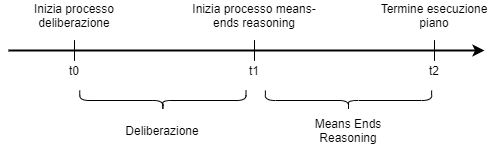
\includegraphics[scale=0.6]{images/deliberazion_meansend_timechart.png}
\end{center}

Definiamo come tempo per deliberare:
\begin{displaymath}
    T_{deliberazione} = t_1 - t_0
\end{displaymath}
\begin{displaymath}
    T_{means-ends-reasoning} = t_2 - t_1
\end{displaymath}

La \textbf{deliberazione è ottimale} se al tempo $t_1$, l’agente ha selezionato l’intenzione da raggiungere che sarebbe stata ottimale se fosse stata raggiunta all’istante $t_0$. A meno che il tempo $T_{deliberazione}$ sia estremamente piccolo, l’agente corre il rischio che l’intenzione selezionata non sia pi`u ottimale nel momento in cui l’agente l’ha deliberata. Ma la fase di deliberazione è solo metà del problema: l’agente deve ancora determinare come realizzare l’intenzione. 

Quindi, \textbf{l’agente avrà un comportamento complessivo ottimale} nelle seguenti circostanze:
\begin{itemize}
    \item Quando il tempo impiegato per i processi di deliberazione e di means-ends reasoning è incredibilmente piccolo.
    \item Quando l'ambiente è garantito rimanere statico mentre l’agente sta eseguendo i processi di deliberazione e di means-ends reasoning.-
    \item Quando un’intenzione ottimale se raggiunta al tempo $t_0$ (momento in cui si osserva l'ambiente) è garantita rimanere ottimale fino al tempo $t_2$ (momento in cui l’agente ha determinato le azioni per raggiungere l’intenzione).
\end{itemize}